\documentclass[10pt, conference, compsocconf]{IEEEtran}

\usepackage{cite}
\ifCLASSINFOpdf
  \usepackage[pdftex]{graphicx}
  % declare the path(s) where your graphic files are
  \graphicspath{{../pdf/}{../jpeg/}}
  % and their extensions so you won't have to specify these with
  % every instance of \includegraphics
  \DeclareGraphicsExtensions{.pdf,.jpeg,.png}
\else
  % or other class option (dvipsone, dvipdf, if not using dvips). graphicx
  % will default to the driver specified in the system graphics.cfg if no
  % driver is specified.
  \usepackage[dvips]{graphicx}
  % declare the path(s) where your graphic files are
  \graphicspath{{../eps/}}
  % and their extensions so you won't have to specify these with
  % every instance of \includegraphics
  \DeclareGraphicsExtensions{.eps}
\fi

% *** FLOAT PACKAGES ***
%
\usepackage{fixltx2e}
% fixltx2e, the successor to the earlier fix2col.sty, was written by
% Frank Mittelbach and David Carlisle. This package corrects a few problems
% in the LaTeX2e kernel, the most notable of which is that in current
% LaTeX2e releases, the ordering of single and double column floats is not
% guaranteed to be preserved. Thus, an unpatched LaTeX2e can allow a
% single column figure to be placed prior to an earlier double column
% figure. The latest version and documentation can be found at:
% http://www.ctan.org/tex-archive/macros/latex/base/

\usepackage{url}
\usepackage[utf8]{inputenc}
\usepackage[T1]{fontenc}
%\usepackage[colorinlistoftodos,textsize=footnotesize,textwidth=1cm]{todonotes}
% \usepackage[disable]{todonotes}
\usepackage{todonotes}
\usepackage{booktabs}
\usepackage{multirow}
\usepackage{array}
\usepackage[cmex10]{amsmath}
\usepackage[caption=false]{subfig}
\usepackage{rotating}
\usepackage{xcolor}
\usepackage{colortbl}
\usepackage[font=footnotesize]{caption}

\newcommand{\viss}{\textsc{V:Issue:lizer} }

\newcolumntype{v}[1]{>{\raggedright \hspace {0pt}}p{#1}}
\def\IEEEbibitemsep{4pt plus 1.6pt}

% correct bad hyphenation here
\hyphenation{op-tical net-works semi-conduc-tor}

% Avoid orphans and widows (thx IEEE help!)
          \clubpenalty = 10000
          \widowpenalty = 10000
          \displaywidowpenalty = 10000

% Balance columns on last page (thx IEEE help!)
          \usepackage{balance}

\begin{document}



% For peer review papers, you can put extra information on the cover
% page as needed:
% \ifCLASSOPTIONpeerreview
% \begin{center} \bfseries EDICS Category: 3-BBND \end{center}
% \fi
%
% For peerreview papers, this IEEEtran command inserts a page break and
% creates the second title. It will be ignored for other modes.
\IEEEpeerreviewmaketitle

% !TEX root = knauss-vissuelizer.tex
\pdfinfo{/Author (Eric Knauss, Daniela Damian) 
/Title (V:issue:lizer: Explore Online Communication) 
/Subject () 
/Keywords (Requirements clarification patterns; distributed requirements engineering; communication of requirements)}

\title{V:issue:lizer\\Explore Online Communication and  Requirements Clarification over Time}


\author{\IEEEauthorblockN{Eric Knauss, Daniela Damian}
\IEEEauthorblockA{SEGAL, University of Victoria, Victoria B.C., Canada\\
knauss@computer.org, danielad@cs.uvic.ca
}}

\maketitle


\begin{abstract}
This demo introduces \viss\ as a tool for exploring online communication and analysing clarification of requirements over time.
\viss\ enables managers to identify hotspots in current development activities, to analyze communication problems, and to identify developers that are knowledgeable about domain or project related issues by offering powerful visualizations.
Our preliminary evaluation shows that \viss\ offers managers valuable information for their decision making.
\end{abstract}

\begin{IEEEkeywords}
requirements clarification patterns; distributed requirements engineering; communication of requirements
\end{IEEEkeywords}

% !TEX root = knauss-vissuelizer.tex
\section{Introduction}

Large software projects are often affected by the need to collaborate across geographically distributed sites and to depend upon online communication to perform requirements related activities. 
More and more teams employ agile approaches that aim at discovering requirements iteratively and rely on frequent communication instead of requirements documentation. 
In such approaches, requirements are defined in the form of user stories, and ongoing discussions around these user stories serve as the main mechanism to clarify the meaning of requirements and to coordinate their implementation \cite{Cao2008}. 
Recording such discussions and decisions in online project repositories is an emerging best practice, not only in large and distributed projects \cite{Aranda2007}.
IBM\textsuperscript{\textregistered}'s Rational Team Concert\textsuperscript{\textregistered} project, with a large distributed team, is an example in which management mandates the recording of all decisions in the project repository for future use in the project\cite{Frost2007}. 
Consequently, online project repositories contain a wealth of requirements-related communication.

In these kinds of environments, however, the expected evolution of a requirement from an initial idea, through clarification, to design and full implementation, often stagnates. 
%Process-related issues, inadequate tool support or inadequate communication [refs) are common reasons for such problems. 
E.g. stakeholders continue to \emph{clarify} the requirement because it is ambiguous, incomplete, or has frequent changes. 
As a result, its implementation can be delayed or sometimes never get started. 
%Bikeshedding, also known as the Parkinson's law of triviality\cite{Parkinson1958} is another common situation in which developers give disproportionate weight and time to solving trivial issues and delay development. 
%An example from the RTC project (jazz.net) is the ongoing discussion of a large number of developers over the  text required in a UI element, and which blocked the development of this user story. 
%Late in the project a manager intervenes and makes a decision "we go with [...] for this iteration", after which development of the story is completed. 
%Although with a happy ending, many situations like this go unnoticed by managers. 
Current requirements management tools offer little support for identifying requirements with progression problems, thereby lowering the project manager's  ability to intervene in a timely manner.

%\begin{figure}[h]
%\begin{center}
%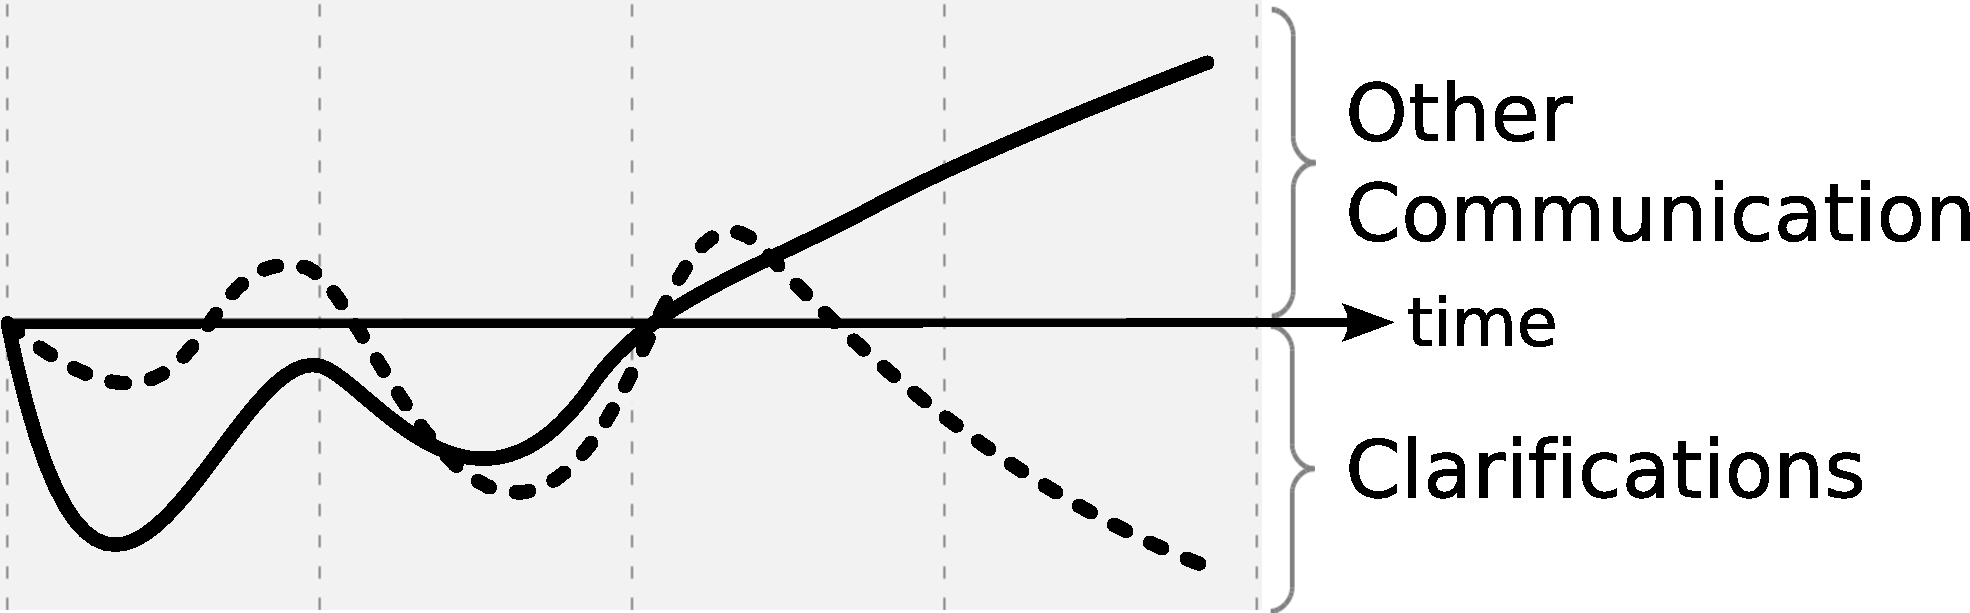
\includegraphics[width=0.7\columnwidth]{img/basic-pattern}
%\caption{Two different trajectories of reqts. communication}
%Predominance of clarifications in requirements-related communication may be problematic }
%\label{fig:basic-pattern}
%\end{center}
%\end{figure}

%Studying recorded online communication fills this gap by offering the potential to reveal patterns of communication that correlate to problematic situations around requirements development. 
In this demo we present a novel tool for analyzing online communication and differentiating between healthy and problematic patterns of communication associated with an individual requirement. 
Our \viss\ tool helps managers to analyze the content of communication among stakeholders involved in the discussion of a particular requirement, identify specific instances of \emph{clarifying} communication, and examine the trajectory of clarifications (i.e. amount of communication and progression) throughout the lifetime of a requirement. 
%Figure \ref{fig:basic-pattern} shows two distinct and quite different possible trajectories of \emph{clarifying} communication in the lifetime of a requirement. 
%While one would expect clarification to diminish as development of a requirement nears the end (solid line trajectory), its predominance throughout the requirement's life may be indicative of problematic requirements (dashed line trajectory). 
%The method proposed in this paper aims to identify these patterns automatically so that managers or involved stakeholders can be made aware of requirements that should be closely investigated.
In addition, \viss\ can visualize social networks that allow to assess the constellation of communication actors and to identify experts for given topics.

%Figure \ref{fig:basic-pattern} depicts the characteristics of clarification communication related to a requirement (here: a story in Jazz).


%The contribution of this paper is the method for the detection and classification of clarification communication patterns, as well as a set of six communication patterns that we identified by applying our method in a large industrial project. 
%The remainder of the paper is structured as follows: Section \ref{sec:relatedwork} surveys related work in the study of communication in requirements engineering (RE), as well as related to information retrieval and automated classification techniques in RE. 
%Section \ref{sec:approach} introduces our research approach in studying requirements communication and the set of our techniques for the detection and classification of clarification  patterns. 
%We then describe the details of the industrial case study in which we applied our techniques in Sections \ref{sec:classification}, \ref{sec:visualization-and-patterns}, \ref{sec:recommendations} and \ref{sec:discussion}, and 
%give a detailed description of the three primary phases of our method: \emph{classification of requirements discussions}, \emph{clarification patterns development} and  \emph{pattern classification}.  
% conclude with future research steps in Section \ref{sec:conclusion}.

%\subsection{Background}
%The Jazz team uses Jazz as collaboration platform. It is the goal of the team to capture the entire communication in comments to \emph{workitems}. One of the workitem types, the \emph{story} contains requirements. Jazz follows an agile development approach, i.e. stories are refined during the project. This includes the decomposition in sub-workitems, most often of the workitem-type \emph{task}. 

%For a given requirement, the graph shows how the amount of clarification changes over time. 
%The example in the figure shows  a reoccurring characteristic that follows one of our six clarification communication patterns: the \emph{perfect clarification} pattern.


%Online communication to perform requirements related activities, such as elicitation, negotiation or development of requirements, is a critical part of large modern software projects. 
%Stakeholders in today's large software projects, most often at geographically distributed sites, largely rely on online communication in their collaboration. 
%Whether they follow an iterative discovery of requirements as in agile projects \cite{Cao2008}, or the time zone differences between stakeholders are too great to allow for frequent synchronous interaction (ref)2, or follow processes that mandate the recording of requirements communication online (ref3), these stakeholders perform various Requirements Engineering related activities through online communication. 

We conducted a preliminary evaluation in two ways. Firstly, we evaluated \viss's ability to correctly identify communication instances concerned with clarification and it's ability to derive meaningful visualizations of the clarification trajectory \cite{Knauss2012f}. 
Secondly, we confronted software managers with \viss's visualizations and asked them, whether the visualization was useful, if it did offer information they would have missed otherwise, and what actions they would perform based on the feedback, if any. 

\begin{figure*}
\centering
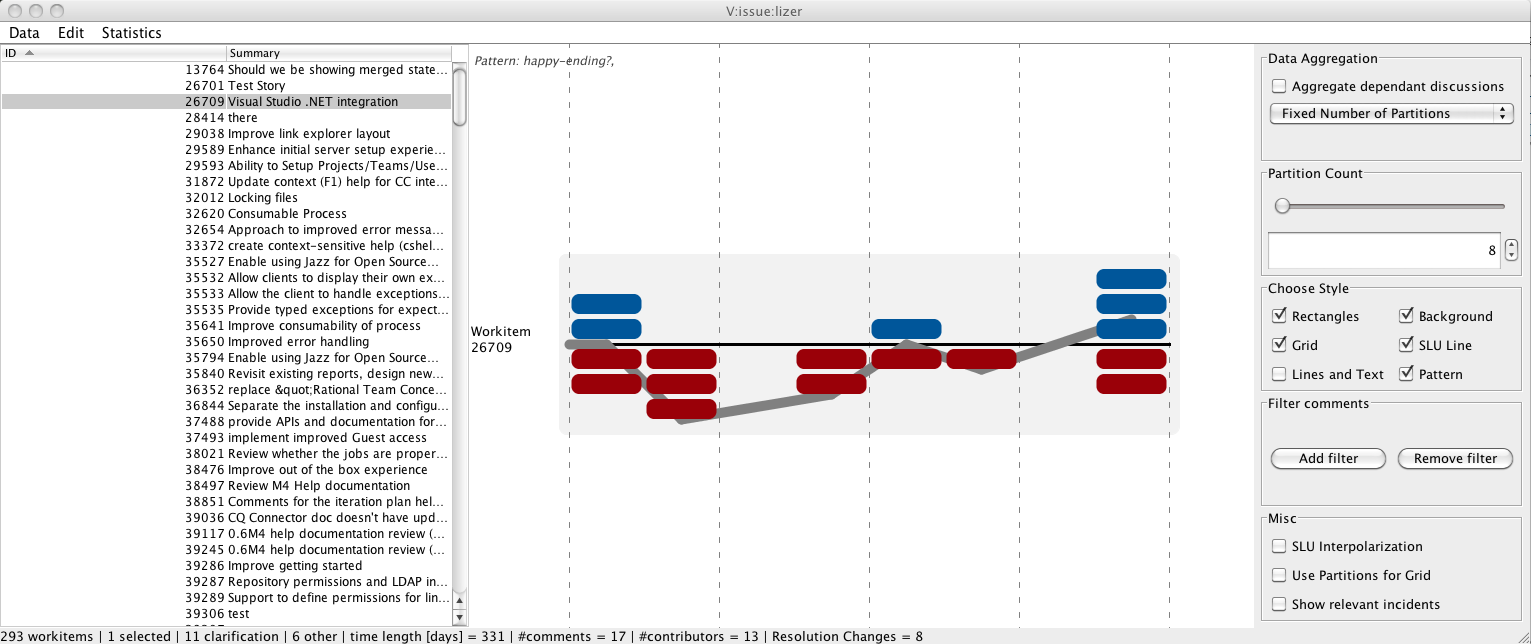
\includegraphics[width=0.8\textwidth]{img/vissuelizer-screenshot}
\caption{Screenshot: the main window of the \viss\ shows a list of issues (e.g. user stories) and their clarification trajectories.}
\label{fig:screenshot}
\end{figure*}
% !TEX root = knauss-vissuelizer.tex
\section{Background and Related Work}
In this paper, we use the term \emph{requirement discussion} to refer to a thread of online communication that is related to a given requirement. 
A requirements discussion consists of \emph{discussion events}, i.e. contributions to the discussion.
We are particularly interested in \emph{clarification events}, i.e. discussion events in which the discussant seeks to improve the understanding of the requirement by either asking for clarification or by offering additional information that clarifies the requirement.
Many software projects use online tools to store requirement discussions, e.g. issue trackers or task management systems like bugzilla, or jira \cite{Ernst2012}. 
In such projects, requirements are distinguished by a certain type of issue (e.g. \emph{user story, enhancement}), and the requirements discussion is stored as a series of comments to this issue.

Issues in such systems crosscut both the technical aspects of a software project and social aspects of collaboration and communication \cite{Kraut1995}. 
Giving managers the ability to find important tasks at the right time can be crucial to project success.
Treude and Storey identified the lack of visualizations as one of the most important short comings of today's task management systems \cite{Treude2010}. 
Accordingly, dashboards that report on the state of a task management system can be pivotal to task prioritization in critical project phases.

Systems like Bugzilla can play a key role in managing software projects, as Ellis et al. \cite{Ellis2007} report, based on results from interviews of how developers use Bugzilla. 
The motivation for their study was the design of a visualization tool that reveals social and historical patterns in tasks.
However, their tool does not support exploring clarification activities.

Many related studies focus on mining and analyzing quantitative data to reveal information about the evolution of the system, or to predict future behaviours but only few works are concerned with visualizing and exploring this information space. 
Treude et al. \cite{Treude2012} present the workitemexplorer, a related tool that allows the exploration of information stored in a task management system.
Compared to this tool, \viss\ allows the analysis of a specialized aspect in this information space, i.e. the analysis of online communication related to clarification of requirements. 
% !TEX root = knauss-vissuelizer.tex
\section{V:Issue:lizer}


\viss\ is an interactive tool that allows software developers and managers to dynamically explore the discussion of requirements  in online repositories with a focus on highlighting the difference between clarification and implementation related communication.


The main window shows a list of requirements on the  left (e.g. workitems in jazz, items in jira, issues in other systems) (see Figure \ref{fig:screenshot}).
\viss\ adds visualizations to the selected discussions in the centre or in an extra window. 
These visualizations help to assess the communication through discussion events (e.g. comments) related to these requirements.
The panel on the right allows users to adjust parameters of the visualization.
Most importantly, the resolution of time intervals for the visualization can be adjusted, either as a fixed number of intervals (here: three and eight intervals), or as a fixed time interval (e.g. days, weeks, month).
%
\viss\ currently supports two different visualizations: 

\subsubsection{Clarification Trajectories} 
This visualization shows how the percentage of clarification events to other discussion events related to a requirement changes over its lifetime.
\begin{figure}[b]
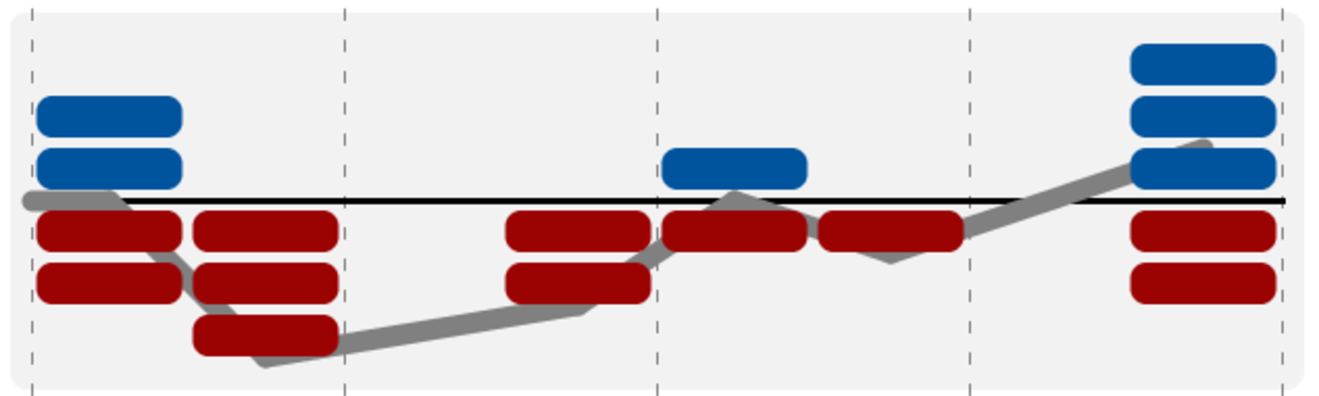
\includegraphics[width=\columnwidth]{img/example-trajectory}
\caption{Example of a requirements discussion's clarification trajectory}
\label{fig:example-trajectory}
\end{figure}
As the visualization of the clarification trajectory (see Figure \ref{fig:example-trajectory}) is a new concept, it needs some explanation.
The black line represents the lifetime of the requirement discussion from the creation of the requirement in the system to the last recorded discussion event.
Dashed lines divide the lifeline into quarters and help to see in which part of the lifetime discussion occurs.
Discussion events are depicted by rectangles.
They are shown below the lifeline, if they are clarification events and above the lifeline if not.
A grey line shows the sum of clarification.
In a classic trajectory with clarification up-front and only implementation related communication in the end, this grey line will start in the bottom left and raise to the upper right corner.
% For increased readability, the different types of discussion events are coloured in the tool (clarification events: red, other: blue).
\viss\ generates these trajectory based on automatic classification of discussion events and identifies reoccurring patterns (\emph{textbook-example, indifferent, discordant, procrastination, back-to-draft, and happy-ending}) \cite{Knauss2012f}.
Typically, there is a number of requirements without pathological findings, e.g. user stories with some clarification in the beginning and other communication events later on that show progress.
More suspicious trajectories show large amounts of clarification late in the iteration, perhaps even after the issue seemed to be solved, or no clarification at all, even though the requirement seems to be complex.
\subsubsection{Social Networks} 
This visualization shows the communication pattern of those participating in a requirement's discussion. 
The developers are presented as nodes; connections between nodes are weighted by the amount of communication both developers share about the requirement in a specific time interval (as defined above) in a requirement's lifetime. 
Thus, subgraphs of the contributors to the discussion in each time interval are created.
Two subgraphs are connected, if  stakeholders appear in several time intervals. 
%Note that subgraphs can be matched to specific time intervals (here: three) where all actors of the subgraph communicate. 
%The interval can be a either a either a fixed number (here: three intervals), or a fixed time interval (e.g. days, weeks, month). 
\viss\ also displays the developer node as a pie chart to show the percentage of clarification vs. implementation-related communication in which the developer is involved (as highlighted in Figure \ref{fig:example-sn-large}).




% integrates information of the automatic analysis of online communication into the social networks, i.e. showing a pie chart with the percentage of clarification and implementation related communication for this developer.


% !TEX root = knauss-vissuelizer.tex
\section{Example Scenarios}
In this section we describe examples that highlight the functionality that \viss\ offers to developers and managers (referred to as users henceforth).

\subsection{Are there problematic requirements?}
%Often, a clear understanding of requirements only evolves during the development of software.
%This is especially true (but not limited to) agile software projects, where managers decide to frame only rudimentary requirements and refine the details on the go.
To identify requirements for which the clarification trajectory indicates potential problems in their development, the user performs the following steps in \viss:

%For a manager, it is important to know when problematic requirements surface, because they can have a serious impact on the project.
%\viss\ helps managers in this scenario as follows:
\begin{enumerate}
\item The user loads a set of requirements (shown as the requirements list on the left panel in Figure \ref{fig:screenshot}).
\item \viss\ automatically analyzes the online communication repository and the discussion related to each of these requirements.  
\item When a requirement is selected from the requirements list its \emph{clarification trajectory} is displayed in the middle panel (see Figure \ref{fig:example-trajectory})
%Discussion events that are concerned with clarifying requirements are depicted by red rectangles below the timeline, other comments are depicted by blue rectangles above the timeline.
\item \viss\ displays suggestive pattern names for the trajectory, e.g. \emph{happy-ending} in Figure \ref{fig:example-trajectory}. This is because the trajectory shows a dominance of clarification even in the second half of the timeline and the grey line only raises above the lifeline in the very end.
\item By scrolling through the list of requirements and associated trajectories the user can make an informed decision, based on this rich information, where to invest more resources to tackle requirements that appear to have problematic development.
\end{enumerate}


\subsection{Are there communication breakdowns?}
Having identified potentially problematic requirements, \viss\  allows the user to more closely investigate who participates in the communication of a requirement (Figure \ref{fig:example-sn} shows the social network for the requirement presented in Figure \ref{fig:example-trajectory}) as follows:
%by After identifying those hotspots, the manager most likely wants to continue with a closer investigation. 
%Often, he or she will investigate who participates in a discussion of a requirement and who is not.
\begin{enumerate}
\item The user opens the social network analysis view.
\item \viss\ displays the social network for the selected requirement.
\item The user analyzes the network and investigates if structural communication problems exist.
\end{enumerate}

\begin{figure}
\centering
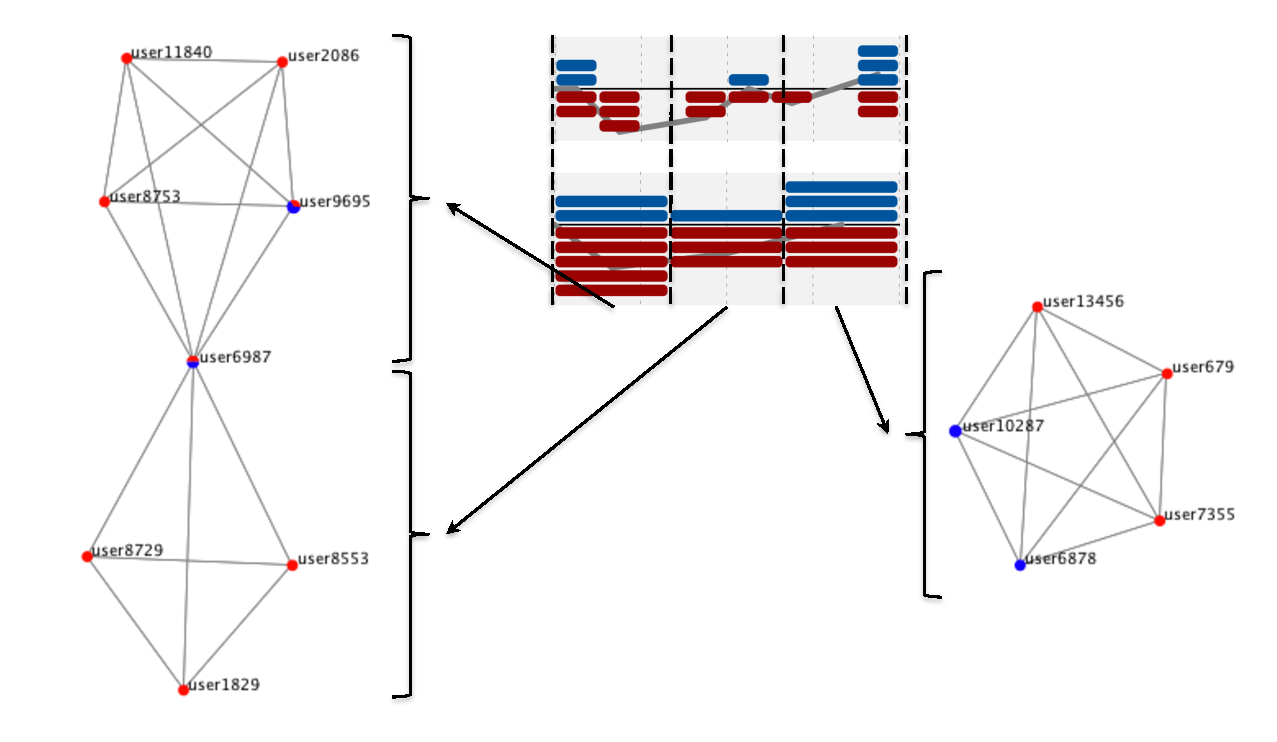
\includegraphics[width=0.8\columnwidth]{img/example-sn}
\caption{Example of a requirements discussion's social network}
\label{fig:example-sn}
\end{figure}

In this example, the user might conclude that there is no single person who is coordinating the analysis and work related to this requirement, because there is no one actor who participates in all relevant time intervals.
The user decides to assign this responsibility to an experienced developer.

\subsection{Who is knowledgeable about a given topic?}

Integrating the right persons into the loop for an important feature is a crucial ability for managers.
To support managers in this task, \viss\ distinguishes between two types of knowledge: (i) domain knowledge that shows in discussion events related to clarification and (ii) implementation specific knowledge that shows in other discussion events.
\begin{enumerate}
\item The user selects a number of requirements that relate to a feature or higher-level topic. 
\item \viss\ creates the social networks generated from requirement discussions and displays them in a single large network (see Figure \ref{fig:example-sn-large}).
\item Based on the pie charts in the social network, the manager identifies candidates with a balanced percentage of clarification and implementation communication.
\item The manager looks for central developers. 
\end{enumerate}
\begin{figure}
\centering
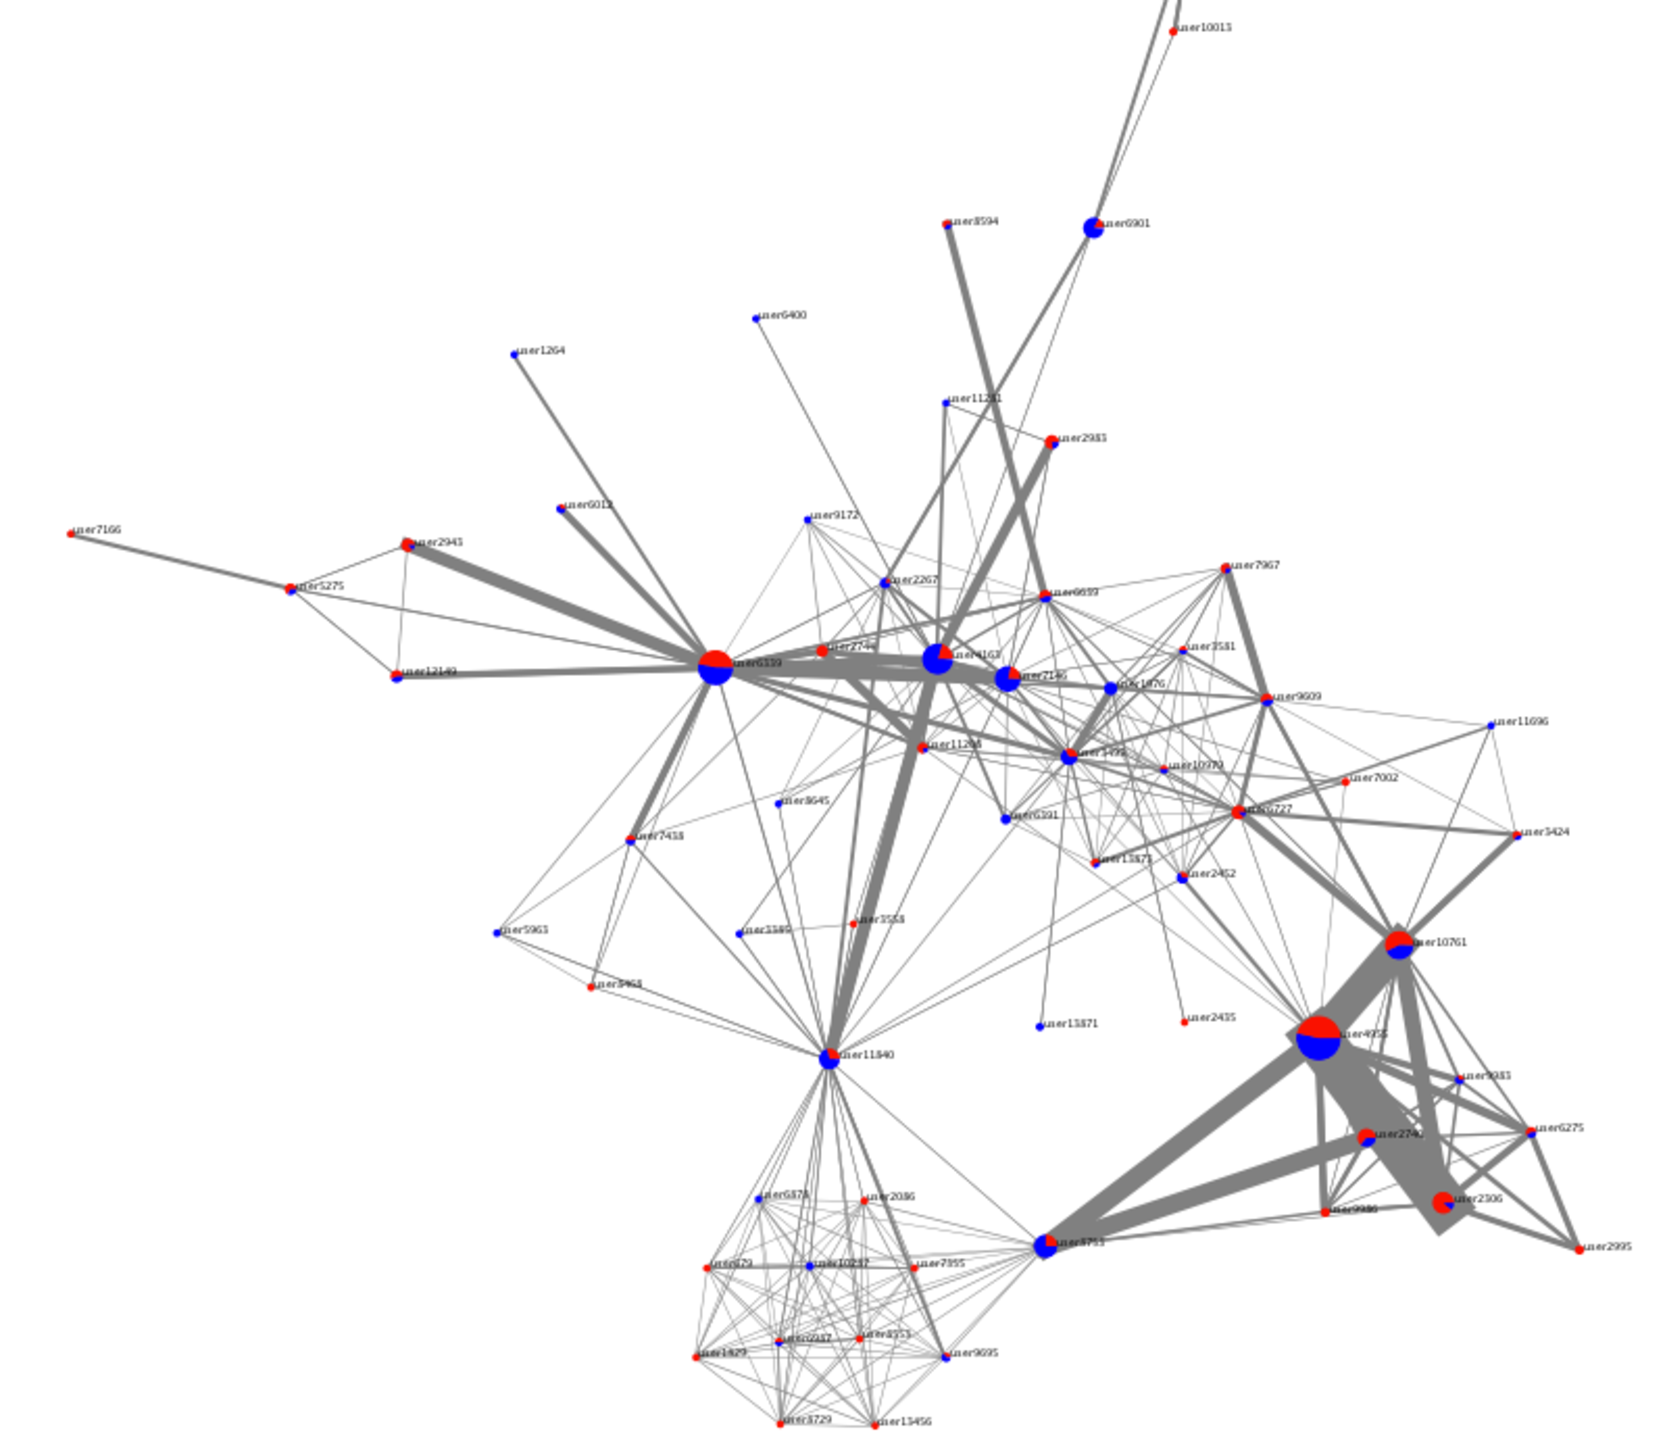
\includegraphics[width=0.8\columnwidth]{img/example-sn-large}
\caption{Example of a social network for a set of requirements discussions}
\label{fig:example-sn-large}
\end{figure}
Central actors with many connections might already have a very high workload, but there exist good candidates that are less central and connect two subnets.

% !TEX root = knauss-vissuelizer.tex
\section{Preliminary Evaluation}
In order to evaluate the \viss and its underlying concepts, we need to investigate several things.
First we need to show that \viss is able to distinguish between communication events that deal with clarification and other events. 
Secondly, we need to determine if and when the feedback from our \viss tool is beneficial for practitioners. 

\subsection{Ability to identify clarification events}
\viss currently uses a Bayesian classifier to identify clarification events, i.e. a supervised machine learning algorithm.
In order to evaluate the ability to identify clarification events, we need to show(i)  that the classifier reaches an acceptable performance with realistic amount of training and (ii) that this performance is sufficient to generate meaningful trajectories on the fly.
We investigated both aspects based on a case study in the IBM Rational Team Concert (RTC) project \cite{Knauss2012f}.
RTC is a globally distributed software project and as such employs online communication to an extend that guarantees a sufficient amount of the overall communication to be available.

In order to provide training data, two raters manually classified ca. 1200 communication events with an acceptable inter-rater agreement.  
Based on this training data, we applied 10-fold cross evaluation and measured a recall of 0.943 and a precision of  0.678, resulting in an acceptable f-measure of 0.789.
Especially the high recall leads to acceptable trajectories that are comparable with those constructed based on manual classification (c.f. discussion in \cite{Knauss2012f}).

\subsection{Ability to support decisions of managers}
We just started to evaluate the ability to support software managers in decision making. 
For a preliminary evaluation, we presented \viss to several software managers, followed by a semi-structured interview.
First, we were able to interview participants of the VIATEC Software Management Round Table, a local group of software managers that regularly meet in Victoria to exchange experiences.
Our interviewees agreed that the clarification trajectories provide significant information to support decisions on resource allocation and risk management. 
In addition, they suggested that the \viss could also support project retrospectives and process improvement efforts. 
The main issue raised by Victoria's software managers was the need of seeing who was participating in a given requirements related discussion. 
Accordingly, a trajectory without clarification would be suspicious if no experienced developer participated in its underlying discussion. 

As an reaction to this feedback, we integrated the ability to generate social networks into \viss and then  talked to managers of the IBM RTC project and related projects for a second round of interviews.
At IBM, our interviewees agreed that the clarification trajectories together with the associated social network graphs are helpful. 
Especially, when the software development reaches the \emph{end game}, i.e. a time close to the release where mostly testing and polishing takes place, clarification events would be very suspicious and would indicate a high risk that needs management attention. 

%\input{recommendations}
%\input{discussion}
% !TEX root = knauss-vissuelizer.tex
\section{Conclusion and Future Work}
\todo[inline]{Dana, please review conclusion}
With \viss\ we introduced a visualization tool to analyze requirements clarification in online communication over time.
Especially agile and distributed projects demand such analysis: agile projects often only sketch requirements in sufficient detail to plan the next iteration and leave the details to be clarified during the development; distributed projects often depend on online communication and challenge their project managers' ability to assess the shared understanding in the team. 
Our preliminary evaluation has shown that our visualizations allow managers to identify hotspots, e.g. user stories that are not clear to the team. 
Furthermore, \viss\ supports managers in investigating the cause of those hotspots and in identifying suitable actions to disarm problematic or risky situations where the team has insufficient understanding of requirements.
 
In future work, we will evaluate how practitioners use our tool in their daily work. 
This will help us to gain further insight on how managers can use information about requirements clarification over time and to quantify the benefits that tools like the \viss\ can offer.

Such further evaluation should also relate features of online communication (i.e. network centrality, late clarification, no clarification) with typical problems of requirements related discussions, such as feature creep \cite{Jones1996} or symmetry of ignorance \cite{Fischer2000}.

\section*{Acknowledgements}
\todo[inline]{There is a number of people we should acknowledge.}
%\vspace{-1cm}
\balance

\listoftodos

\bibliographystyle{IEEEtran}
\bibliography{IEEEabrv,bibliography}
\end{document}
